% !TEX encoding = UTF-8 Unicode

\documentclass[a4paper]{article}

\usepackage{color}
\usepackage{url}
\usepackage[utf8]{inputenc} % make weird characters work
\usepackage{graphicx}

\usepackage{amsmath}
\usepackage{tcolorbox}
%Milica: meni ne radi ovde serbian, samo croatian :(
\usepackage[english,croatian]{babel}


\usepackage[unicode]{hyperref}
\hypersetup{colorlinks,citecolor=green,filecolor=green,linkcolor=blue,urlcolor=blue}
%\newtheorem{primer}{Пример}[section] %ćirilični primer
\newtheorem{primer}{Primer}[section]
\newtheorem{definicija}{Definicija}[section]

\begin{document}

\title{Formalna semantika programskih jezika\\ \small{Seminarski rad u okviru kursa\\Metodologija stručnog i naučnog rada\\ Matematički fakultet}}

\author{Isidora Đurđević, Ana Stanković,\\
 Milica Đurić
\\isidoradjurdjevic.100@gmail.com, anastankovic167@gmail.com,\\
 mdjuric55@gmail.com}

\date{15.~april 2017.}
\maketitle

\abstract{
Semantika ima posebnu ulogu u teoriji i proučavanju značenja programskih jezika. Cilj ovog rada je da pokaže koja je uloga formalnog zadavanja semantike programskih jezika i osnovne primene formalne semantike. Biće definisana tri osnovna pristupa semantike: operaciona, denotaciona i aksiomatska semantika i objašnjene njihove uloge. Svaki od pristupa je potkrepljen primerom koji prikazuje primenu te semantike u računarstvu.

\textit{Ključne reči}: Semantika programskih jezika, formalna semantika, operaciona semantika, denotaciona semantika, značenje programa.

\tableofcontents

\newpage

\section{Uvod}
\label{sec:uvod}

\qquad Vođenje konverzacije ne bi bilo moguće bez znanja o tome šta koja reč koju koristimo predstavlja. U našoj glavi stoje jasne neformalne definicije svake reči koje znamo i pomoću kojih povezujemo objekte sa njihovim značenjem. U lingvistici, nauci o jeziku, svaka reč dobija svoju formalnu definiciju, a pravila formiranja rečenica su jako rigorozna, odnosno, postoje jasne odredbe šta je ispravno, a šta neispravno. Ove formalne definicije i pravila omogućavaju onima koji se susreću sa jezikom po prvi put da ga lakše nauče i razumeju kako bi mogli da ga koriste. Slično, ovo može biti primenjeno i na programske jezike.

 Kao što je izučavanje prirodnog jezika podeljeno  na izučavanje strukture onoga čime se nešto izražava, tj. \textit{sintakse} i izučavanje značenja onoga što je izraženo, tj. \textit{semantike}, tako se i proučavanje programskog jezika može podeliti na proučavanje njegovog formiranja i njegovog značenja. Osnovni zadatak sintakse programskih jezika je da omogući formiranje korektnih programa iz ugla strukture izraza. Izrazi poput $ x++; function(x,y); $ su sintaksno ispravni, ali šta oni predstavljaju, koje je njihovo značenje? Sintaksa nema odgovor na ovo pitanje jer ona nije povezana sa značenjem ili ponašanjem programa u toku izvođenja, to je zadatak \textit{\textbf{semantike programskih jezika}}. Međutim, sintaksa mora biti definisana pre semantike jer se značenje može pridružiti samo ispravnim izrazima jezika. Definisanje sintakse je obično lakši posao od definisanja semantike.

	Semantika može da se opiše formalno i neformalno, gde je češće neformalno opisivanje, odnosno opisivanje prirodnim jezikom što može biti neprecizno. Zato se u narednim glavama bavimo formalnim opisom semantike koja bi trebalo da otkloni sve nepreciznosti i da d\^a potpunu definiciju programskog jezika. Biće opisani neki od formalnih pristupa kao što su \textit{operaciona, denotaciona i aksiomatska} semantika. Svakom od pristupa će se prići površinski zbog same složenosti formalnog definisanja, a čitaocu se ostavlja da proširi svoje znanje u naznačenoj literaturi.



\section{Formalna semantika}
\label{sec:forsem}

\qquad Kao što je već napomenuto, semantika se može definisati formalno i neformalno. Pri neformalnom definisanju koristimo prirodan jezik. Na primer, izraz $ while(x > 0)$  $\lbrace x--;\rbrace$ može se opisati rečima : "sve dok je vrednost promenljive x veća od nule umanjuj vrednost promenljive x za jedan". Ovaj zadatak postaje teži sa pojavom veće kompleksnosti programskog koda.

Teško je pisati vrlo precizne definicije neformalnim jezikom, obično postane komplikovano za razumeti i predugačko za neke kompleksne programske jezike što dovodi do loše napisanih programa jer se stvaralac programskog jezika i onaj ko ga koristi ne razumeju. To je jedan od razloga zašto se uvodi \textit{formalna semantika}, što znači precizna semantika.

Pri učenju novog programskog jezika, programer bi trebalo da uči i samu logiku jezika. Neki vid opisa logike programskog jezika olakšava programerima pisanje jakih i stabilnih programa.  Ovaj opis nam može pružiti, takođe, formalna semantika.

Još jedan od razloga zašto se uvodi formalna semantika jeste to što ona čini osnovu formalne verifikacije programa, tj. deo je interpretera i kompajlera. Na slici \ref{fig:kompajler} dat je prikaz kompajlera.

\begin{figure}[h!]
\begin{center}
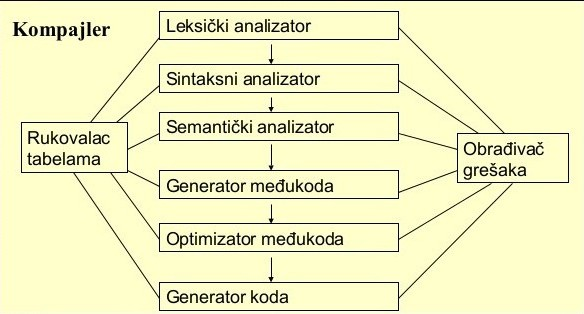
\includegraphics[scale=0.5]{kompajler.jpg}
\end{center}
\caption{Struktura kompajlera \cite{slika}}
\label{fig:kompajler}
\end{figure}

Kompleksnost uvođenja formalne semantike daje više načina pristupa njenom definisanju. Mi ćemo se fokusirati na tri pristupa:
\begin{enumerate}
  \item \textbf{Operaciona semantika}

  Značenje programa predstavlja tok koraka izvršavanja programa sa datim ulazom.
  \item \textbf{Denotaciona semantika}

  Značenje programa je matematička funkcija koja prevodi ulaz u izlaz programa.
  \item \textbf{Aksiomatska semantika}

  Značenje programa je ono što može biti dokazano o njemu koristeći aksiome.
\end{enumerate}

U sledećim poglavljima, svaka od ovih formalnih semantika će biti opisana šire.
\section{Operaciona semantika}
\label{sec:opsem}

\qquad Operaciona semantika je način davanja značenja programskim jezicima kroz matematičku reprezentaciju. Svrha operacione semantike je da opiše \textit{kako} se izvršavaju programi, ne samo koji su rezultati izvršavanja tog programa. Preciznije, ona treba da opiše kako se stanja menjaju tokom izvršavanja naredbe programa. U okviru ove semantike postoje:
\begin{itemize}
	\item \textit{Prirodna semantika} (ili veliki koraci (eng.~{\em big-step semantics})): svrha joj je da opiše kako su \textit{ukupni rezultati} izvršavanja dobijeni.
	\item \textit{Strukturna operaciona semantika} (ili mali koraci (eng.~{\em small-step semantics})): svrha joj je da opiše kako se \textit{svaki korak} izvršava.
\end{itemize} \cite{wiley}.

Ponašanje se formalno može definisati korišćenjem apstraktnih mašina, formalnih automata, tranzicionih sistema... U daljem tekstu ćemo prikazati primer korišćenja apstraktne mašine za definiciju, kao i upotrebu tranzicionih sistema.\\
Za svaki programski jezik možemo definisati realnu ili apstraktnu mašinu, na kojoj ćemo pratiti promene stanja koje proizvode pojedini konstrukti programskog jezika. Ovako definisana mašina biće interpretator određenog programskog jezika. Naravno, za ovo nije dobro izabrati realnu mašinu, jer bi semantičke definicije bile vezane za jednu konkretnu mašinu, a to znači i za sve specifičnosti određene arhitekture računara. Zato je izbor apstraktne mašine pogodniji. Pokazaćemo ovo na jednom primeru. Posmatrajmo brojački programski ciklus u jeziku Pascal:\\

\begin{center}\textit{for i:= početak to kraj do}
\\.
\\.
\\.
\end{center}
\hfill \break
Značenje ovakvog zapisa ne može biti lako razumljivo. Stvarni mehanizam izvršavanja ciklusa je skriven za korisnika. Naravno, oni koji poznaju razne zapise programskih ciklusa mogu lako pretpostaviti značenje gore navedenog zapisa. Međutim, i za njih će biti teško da odgovore, šta će se dogoditi ako je vrednost promenljive \textit{početak} veća od vrednosti promeljive \textit{kraj}?\\
\\Zamislimo sada da naša apstraktna mašina raspolaže instrukcijama dodele, uslovnog i bezuslovnog prelaska. Tada bi se gore navedeni ciklus mogao zapisati instrukcijama apstraktne mašine u obliku:\\

\hspace{4cm} \textit{i:=početak}\\
\textit{ciklus:} \hspace{3cm} \textit{if i \textgreater kraj then goto izlaz}
\begin{center}
.
\\.
\\.
\\ \textit{i:=i+1}
\\ \textit{goto ciklus}
\end{center}
\textit{izlaz:} \hspace{4cm} ...\\
\\Sada je jasno značenje programskog ciklusa, pa i to da se telo ciklusa neće izvršiti ako je vrednost promenljive \textit{početak} veća od vrednosti promenljive \textit{kraj}.\\
\\Ovo objašnjenje nam daje apstraktnu definiciju \textit{kako} se program izvršava na mašini. Bitno je primetiti da jeste zaista apstrakcija: ignorišemo detalje kao što je upotreba registara i adresa za promenljive. Dakle, operaciona semantika je nezavisna od arhitekture mašine i načina implementacije.\\

Opišimo sada značenje koje se predstavlja na isti način za obe vrste operacione semantike, prirodne i strukturno operacione, \textit{tranzicionim sistemom} na primeru rada \emph{While} petlje. Ona će imati dve vrste konfiguracija \cite{willey}:
\begin{itemize}
	\item $\langle$ S, s $\rangle$ - Naredba \textit{S} će biti izvršena od stanja \textit{s}.
	\item s predstavlja završno stanje.
\end{itemize}
\textit{Tranziciona relacija} će onda opisivati kako izgleda tok izvršavanja. \\

U prirodnoj semantici je bitna veza između početnog i završnog stanja izvršavanja. Tada će tranziciona relacija prikazivati vezu između početnog stanja i završnog stanja za svaku naredbu. Tranziciju ćemo obeležavati kao

\begin{center}$\langle$ \textit{S, s} $\rangle$ $\rightarrow$ \textit{s'} \end{center}
Intuitivno ovo znači da izvršavanje \textit{S} iz \textit{s} će se završiti i rezultujuće stanje će biti \textit{s'}.

Definiciju za  $\rightarrow$ možemo videti u tabeli ~\ref{tab:b}. \textit{Pravilo} generalno ima formu

\begin{center}$\frac{\langle S_1, s_1 \rangle \rightarrow S'_1, s'_1, ... , \langle S_n, s_n \rangle \rightarrow s'_n}{\langle S, s \rangle \rightarrow s'}$ \end{center}

gde \textit{$S_1$, ..., $S_n$} nazivamo neposrednim konstituentima od \textit{S}. Pravilo se sastoji iz određenog broja \textit{premisa} (nalazi se iznad linije) i jednog \textit{zaključka} (nalazi se ispod linije).

Pravilo takođe može imati određeni broj \textit{uslova} (nalazi se sa desne strane linije) koji moraju biti ispunjeni kako bi se primenilo pravilo. Pravilo sa praznim skupom premisa se naziva \textit{aksiom}. \cite{willey}

\begin{table}[h]
       \caption{Prirodna semantika za While petlju}
    	\begin{center}
        \begin{tabular}{lrc}\hline
        \hline
        \hline
        $[ass_{ns}] $ & $ \langle x := a, s \rangle \rightarrow s[x \mapsto A[[a]]s]$    \\  [6pt]
        $[skip_{ns}] $ & $ \langle skip, s \rangle \rightarrow s$   \\ [6pt]
         $[comp_{ns}] $ & $ \frac{\langle S_1, s \rangle \rightarrow s', \langle S_2, s' \rangle \rightarrow s''}{\langle S_1;S_2, s \rangle \rightarrow s''}$ \\[6pt]
            $[if^{tt}_{ns}] $ & $ \frac{\langle S_1, s \rangle \rightarrow s'}{\langle if\ b\ then\ S_1\ else\ S_2,\ s \rangle \rightarrow s'}\  if\ B[[b]]s\ =\ tt $ \\ [6pt]
            $[if^{ff}_{ns}] $ & $ \frac{\langle S_2, s \rangle \rightarrow s'}{\langle if\ b\ then\ S_1\ else\ S_2,\ s \rangle \rightarrow\ s'}\  if\ B[[b]]s\ =\ ff $ \\ [6pt]
            $[while^{tt}_{ns}] $ & $ \frac{\langle S, s \rangle \rightarrow s', \langle\ while\ b\ do\ S,\ s' \rangle \rightarrow\ s''}{\langle\ while\ b\ do\ S,\ s \rangle \rightarrow\ s''}\ if\ B[[b]]s\ =\ ff $ \\ [6pt]
             $[while^{ff}_{ns}] $ & $ \langle\ while\ b\ do\ S,\ s \rangle \rightarrow\ s\ if\ B[b]s\ =\ ff$ \\ [6pt]
          \hline \hline
        \end{tabular}
     \label{tab:b}
    \end{center}
\end{table}

Kada se koriste aksiomi i pravila da se izvede tranzicija $\langle$ \textit{S, s} $\rangle$ $\rightarrow$ \textit{s'} dobija se \textit{stablo izvođenja}. \textit{Koren} stabla izvođenja je upravo $\langle$ \textit{S, s} $\rangle$ $\rightarrow$ \textit{s'}, dok su listovi instance aksioma. Unutrašnji čvorovi su zaključci instanciranih pravila i njihova neposredna deca će biti odgovarajuće premise. Stablo izvođenja se naziva \textit{jednostavnim stablom} ako je instanca aksioma, inače se naziva \textit{kompozitnim stablom}.\\

\begin{primer}
(z := x, x := y); y := z \\
Neka $s_0$ bude stanje koje mapira sve promenljive osim x i y u 0 i ima $s_0$ x = 5 i $s_0$ y = 7. Tada dobijamo sledeće stablo izvođenja:

\begin{center}$\frac{\frac{\langle z := x, s_0 \rangle \rightarrow s_1\ \ \langle x := y, s_1 \rangle \rightarrow s_2}{\langle z := x, x := y, s_0\rangle \rightarrow s_2\ \ \langle y := z, s_2 \rangle \rightarrow s_3}}{\langle (z := x; x := y); y := z, s_0 \rangle \rightarrow s_3}$ \end{center}

\end{primer}

Posmatrajmo problem konstruisanja stabla izvođenja za datu naredbu \textit{S} i stanje \textit{s}. Najbolji pristup ovakvom problemu jeste konstruisati stablo od korena \textit{nagore}. Dakle, počinjemo pronalaskom aksioma ili pravila sa zaključkom gde se leva strana slaže sa konfiguracijom $\langle$ \textit{S, s} $\rangle$. Imaćemo dva slučaja:
\begin{itemize}
	\item Ako je u pitanju aksiom i ako su uslovi aksioma ispunjeni onda možemo da zaključimo završno stanje i konstrukcija stabla izvođenja je gotova.
	\item Ako je u pitanju pravilo, sledeći korak je pokušati konstruisati stablo izvođenja za premise datog pravila. Kad se ovaj deo odradi, neophodno je proveriti da li su uslovi pravila ispunjeni i tek onda možemo zaključiti završno stanje  $\langle$ \textit{S, s} $\rangle$.
\end{itemize}
%primer stabla

\section{Denotaciona semantika}
\label{sec:densem}

\qquad Nastala 1960. godina od strane Christopher Strachey-a i njegove istraživačke grupe na Oxford-u \cite{slonneger1995book}, \textit{denotaciona semantika} predstavlja jednu vrstu reakcije na operacionu semantiku za koju se smatra da sadrži puno informacija. Naziv je dobila po engleskoj reči označiti (eng.~{\em denote}) jer pridružuje značenja sintaksnim definicijama jezika. Alternativno, može se nazivati i \textit{matematička semantika} zbog njene okrenutosti matematičkim formalizmima pri definisanju ove formalne semantike. Jedan način definisanja denotacione semantike je dat u sledećoj definiciji.
\begin{definicija}
Pristup formalizaciji semantike konstruisanjem matematičkih objekata koji
opisuju značenje jezika naziva se \textbf{denotaciona semantika} \cite{milena}.
\end{definicija}

Dok se u operacionoj semantici vodilo računa o koracima izvršavanja, u denotacionoj to postaje nebitno. Na primer, značenje izraza $ (15+3)*(2+2) $ jeste 72 i ne treba obraćati pažnju na unutrašnja izračunavanja. Bitan je samo efekat koji izvršavanje programa proizvodi, odnosno odnos između početnog i završnog stanja programa. Za posmatranje ovog efekta potrebno je uočiti odnos između sintakse i semantike programskog jezika.

Ideja ove semantike je da poveže svaki deo programskog jezika sa nekim matematičkim objektom kao što je broj ili funkcija. Odavde se jasno vidi da je potrebno raščlaniti programski jezik na sintaksne delove (to nam pruža apstraktna sintaksa) i svakom delu dodeliti značenje. Svaka sintaksna definicija se tretira kao objekat na koji se može primeniti funkcija koja taj objekat preslikava u matematički objekat koji definiše značenje \cite{parezanovic}. Dodeljivanjem značenja delovima programa dodeljuje se značenje celokupnom programu što nam govori o najvažnijem aspektu denotacione semantike.
\begin{definicija}
Semantika jedne programske celine definisana je preko semantike njenih poddelova. Ova osobina denotacione semantike naziva se \textbf{kompozitivnost}.
\end{definicija}

Ovo znači da ukoliko se zameni jedan deo programske celine sa delom koji ima isto značenje, neće se promeniti značenje cele programske celine. Gore pomenuti izraz je imao semantičku vrednost 72, a to isto značenje ima i izraz $ (16+2)*(2+2) $. To znači da se semantika izraza nije promenila iako su zamenjeni delovi izraza. Nije došlo do promene jer $ 15+3 $ ima isto značenje kao i $ 16+2 $. Treba se još pozabaviti dodeljivanjem semantičke vrednosti delovima programske celine.

Nekim sintaksnim delovima programa je lako dodeliti semantičku vrednost. Takvi su brojevi ili aritmetički operatori jer oni već imaju svoje matematičko značenje. Ali neke sintaksne definicije poput rekurzije ili goto naredbe je teško videti kroz matematičko značenje. Daćemo primer definisanja denotacione semantike aritmetičkih izraza, dok se o rekurziji ili nekim naprednijim primerima može pročitati više u \cite{nielson}.\\


Potrebno je prvo definisati apstraktnu sintaksu aritmetičkih izraza. Neka su podržani samo prirodni brojevi i od aritmetičkih operatora +. Ovo znači da će semantička vrednost nekog izraza biti prirodan broj. Primer definicije apstraktne sintakse ovakvih aritmetičkih izraza dat je u nastavku.


\begin{tcolorbox}
\textbf{Sintaksni domeni i pravila:}
\\

$B: Broj $  \qquad\qquad Nenegativan broj

$C: Cifra $ \qquad\qquad Cifra 0,1...,9

$I: Izraz $

$ Broj ::== Cifra | Broj Cifra $

$ Cifra ::== 0 | 1 | 2 | 3 | 4 | 5 | 6 | 7 | 8 | 9 $

$ Izraz ::== Broj | Izraz+Izraz $
\end{tcolorbox}

Sledeći korak jeste definisanje matematičkih objekata koji će predstavljati semantičke vrednosti.  Ti matematički objekti nazivaju se \textbf{semantički domeni}. Njihova kompleksnost zavisi od toga koliko je kompleksan programski jezik kojem dajemo značenje. U našem jednostavnom primeru, kao što je već rečeno, semantička vrednost može biti samo prirodan broj.
\begin{tcolorbox}
\textbf{Semantički domeni}
\\

$N={0,1,2,3,....} $  \qquad\qquad Skup prirodnih brojeva

\end{tcolorbox}
Posle uvedenih objekata, treba uvesti neke matematičke funkcije koje će davati značenje prethodno uvedenim sintaksnim definicijama. Takve funkcije se nazivaju \textbf{funkcije značenja }(eng.~{\em meaning functions}). Definicije funkcija koje su potrebne za naš jednostavan primer su date u nastavku.
\begin{tcolorbox}
\textbf{Funkcije značenja}
\\

$povezibn: B \rightarrow N $  \qquad Unarna funkcija - povezuje broj sa N

$povezicn: C \rightarrow N $  \qquad Unarna funkcija - povezuje cifru sa N

$semantika: I \rightarrow N $   \qquad Unarna funkcija - povezuje izraz sa N

$plus: N \times N \rightarrow N $  \qquad Binarna funkcija plus - isto što i +

$pom: N \times N \rightarrow N $ \qquad Binarna funkcija pom - isto što i *

$ povezicn[[0]] = 0,... ,povezicn[[9]] = 9 $

$ povezibn[[D]] = povezicn[[D]] $

$ povezibn[[B D]] = plus(pom(10, povezibn[[B]]),povezibn[[D]]) $

$ semantika[[B]] = povezibn[[B]] $

$ semantika[[I1 + I2]] = plus(semantika[[I1]],semantika[[I2]]) $

\end{tcolorbox}
Primetimo da su korišćene zagrade $ [[,]]$ koje imaju ulogu da razdvoje semantički deo od sintaksnog dela. U okviru zagrada nalazi se sintaksni deo definicija. Primer koji oslikava korišćenje denotacione semantike je dat u nastavku.
\begin{primer}
Pronaći značenje izraza 2+32+61.

Rešenje:
\begin{center}
\textbf{semantika[[2+32+61]]} = plus(semantika[[2+32]],semantika[[61]])\\
= plus(plus(semantika[[2]],semantika[[32]]),povezibn[[61]])\\
= plus(plus(2,32),61)\\
= plus(2+32,61)\\
= plus(34+61) = 34+61 = 95
\end{center}

jer je:

\begin{center}
\textbf{semantika[[2]]} = povezibn[[2]] = povezicn[[2]] = 2
\end{center}
\begin{center}
\textbf{semantika[[32]]} = povezibn[[32]]\\
= plus(pom(10,povezibn[[3]]),povezibn[[2]])\\
=plus(pom(10,povezicn[[3]]),povezicn[[2]]) \\
=plus(pom(10,3),2) = plus(10*3,2)\\
= plus(30,2) = 30+2 = 32\end{center}

\begin{center}
\textbf{semantika[[61]]} = povezibn[[61]] \\
=plus(pom(10,povezibn[[6]]),povezibn[[1]])\\
=plus(pom(10,povezicn[[6]]),povezicn[[1]]) \\
=plus(pom(10,6),1) = plus(10*6,1)\\
= plus(60,1) = 60+1 = 61

\end{center}
\end{primer}

 Prednost denotacione semantike je u tome što apstrahuje kako se programi izvršavaju. Analiziranje programa se svodi na analiziranje matematičkih objekata, što olakšava stvar. Denotaciona semantika ima veliku primenu u konstrukciji programa za prevođenje \cite{parezanovic}.

\section{Aksiomatska semantika}
\label{sec:akssem}
\qquad Za nastanak i razvoj \textit{aksiomatske semantike}  su zaslužni pre svega Robert Flojd (eng.~{\em  Robert Floyd}), Toni Hor (eng.~{\em  Antony Hoare}) i Edsger Dijkstra (hol.~{\em Edsger Dijkstra}).
 Zasniva se na matematičkoj logici pa je kao takva apstraktnija od denotacione i operacione sematike. Ova semantika
 značenje programa zasniva na tvrdnjama o vezama koje ostaju iste svaki put kad se program izvrši \cite{slonneger1995book}.
 Aksiomatska semantika razvija metode za proveru korektnosti programa. Za svaku kontrolnu strukturu i komandu se definišu logički izrazi. Ovi izrazi se nazivaju \textbf{tvrđenja} (eng.~{\em  assertions}) i u njima se zadaju ograničenja za promenljive koja se javljaju u tim kontrolnim strukturama i komandama.

\begin{tcolorbox}
Tvrđenja su data u obliku Horovih trojki:

  \center \textbf{\{P\}c\{Q\}}

\end{tcolorbox}




\begin{definicija}
\textbf{Horova trojka \{P\}C\{Q\}} opisuje kako izvršavanje dela koda menja stanje izračunavanja ako je ispunjen preduslov (eng.~{\em  precondition}) \{P\}, izvršavanje komande C vodi do postuslova (eng.~{\em  postcondition}) \{Q\} \cite{milena} .

\end{definicija}

Preduslov je logički izraz u kome se definišu ograničenja promenljivih pre izvršavanja komande, a postuslov definiše ograničenja promenljivih posle izvršavanja komande.
Horove trojke se drugačije nazivaju i \textit{delimična ispravnost specifikacije } (eng.~{\em  partial correctness specification}) .
Ali one ne mogu da osiguraju da će se program završiti pa se zbog toga i nazivaju “delimičnim”.

Delimične ispravnosti tvrdnje će biti određene sistemom zaključivanja koji se sastoji iz skupa aksioma i pravila. Za sve konstruktore jednostavnog imperativnog programskog jezika, Horova logika obezbeđuje aksiome i pravila izvođenja \cite{milena}. Aksiomatski sistem za delimičnu ispravnost je dat u Tabeli ~\ref{tab:a} ispod.

\begin{table}[h]
  \caption{Aksiomatski sistem za delimičnu ispravnost}\label{tab:a}
    \begin{center}
        \begin{tabular}{lrc}\hline
        \hline
        \hline
        $[ass_{p}] $ & $ \{ P[x \rightarrow [\![A]\!]\} x:= a \{P\}$    \\  [6pt]
        $[skip_{p}] $ & $ \{P\}$ skip  $ \{P\}$   \\ [6pt]
         $[comp_{p}] $ & $  \frac{\{P\}S_1\{Q\},\{Q\}S_2\{R\}}{\{P\}S_1;S_2\{R\}} $ \\[6pt]
            $[if_{p}] $ & $  \frac{\{B[\![b]\!]\land P\}S_1\{Q\},\{\neg B[\![b]\!]\land P\}S_1\{Q\}}{\{P\} if b then S_1 else S_2\{Q\}} $ \\ [6pt]
        $[while_{p}] $ & $  \frac{\{B[\![b]\!]\land P\}S\{P\}}{\{P\} while b do S \{\neg B[\![b]\!]\land P\}} $ \\ [6pt]
          $[cons_p{p}] $ & $  \frac{\{P^{'}\}S\{Q^{'}\}}{\{P\}S\{Q\}} $ if $ P \Rightarrow	 P^{'} $ and $ Q \Rightarrow	 Q^{'} $  \\ [6pt]
          \hline \hline
        \end{tabular}
    \end{center}
\end{table}






Pored delimične ispravnosti specifikacije, imamo i \textit {potpunu ispravnost naredbe } (eng.~{\em  total correctness statements}) koja osigurava da će se program završiti dok god preduslov važi.

Pored dokazivanja korektnosti programa i algoritama, uloga aksiomatske sematike je i dokazivanje ispravnosti harverdskih opisa (ili nalaženje bagova), proširena statička provera (npr. provera granice niza), dokumentacija programa i interfejsa.

Preduslovi i postuslovi mogu se smatrati interfejsom ili ugovorom između programa i njegovih klijenata. Oni pomažu korisnicima da razumeju šta program treba da proizvede bez potrebe da shvati kako se program izvršava. Tipično, programeri ih pišu kao komentare za funkcije i
funkcionišu kao dokumentacija i olakšavaju održavanje programa. Takve specifikacije su posebno
korisne za bibliotečke funkcije za koje izvorni kod često nije dostupan korisnicima \cite{adrian}.

Način funkcionisanja ove semantike možemo prikazati u primeru sa faktorijalom koji sledi (primer je preuzet iz knjige \cite{nielson} ). \\
\begin{primer}
$\{ x=n \} $ \\
$  y := 1; $
 while $ \neg(x=1) $  do $ (y := x*y; x := x-1) $\\
$ \{ y=n!$ and $ n > 0 \} $ \\

n je u primeru specijalna promenljiva koja se naziva logička promenljiva i koja, za razliku od programskih promenljivih, ne sme se pojaviti ni u jednoj naredbi koja se izvršava u programu i njena vrednost će uvek biti ista. Njena uloga je da pamte inicijalne vrednosti programskih promenljivih. \\
 Zapisali smo  preduslov da promenljiva n ima jednaku vrednost kao i x u početnom stanju (tj. nego što program sa faktorijalom krene da se izvršava). S obzirom da program neće promeniti vrednost promenljive n, postuslov y=n! će izraziti da konačna vrednost y  će biti jednaka faktorijalu početne vrednosti promenljive x, kada se izvršavanje programa završi. \\

\end{primer}

\section{Zaključak}
\label{sec:zakljucak}

Prilikom izučavanja programskih jezika treba obratiti pažnju kako na sintaksu, tako i na semantiku. Sintaksa nam daje skup pravila zapisivanja jezika, dok semantika daje značenje tim konstrukcijama, odnoso programa u celini. Cilj \textit{formalnog} opisa semantike bio bi da se isključe sve nepreciznosti koje može da proizvede primena prirodnog jezika u opisu semantike programskog jezika. Na tri načina je moguće opisati formalnu semantiku programskih jezika: \textit{operacionom, aksiomatskom  i  denotacionom semantikom}. Operaciona semantika opisuje \textit{kako} se izračunavanje izvršava i u okviru ove semantike postoje strukturna operaciona semantika i prirodna operaciona semantika. Aksiomatska semantika je zasnovana na matematičkoj logici i osnovni motiv za opis semantike jezika na ovaj način jeste razvoj metoda za proveru korektnosti programa. Denotaciona semantika sastoji se u pridruživanju značenja sintaksnim definicijama jezika. Primena formalnih opisa semantike zahteva matematičko znanje i apstraktno razmišljanje.


\addcontentsline{toc}{section}{Literatura}
\appendix
\bibliography{seminarski}
\bibliographystyle{plain}

\appendix

\end{document}
